\begin{surferPage}[Cúspide A2+-]{Una cúspide (singularidad $A_2^{+-}$)}
La siguiente ecuación corresponde a una \emph{cúspide} o
 \emph{singularidad cuspidal}:
    \vspace*{-0.4em}
    \begin{center}
      $x^3+y^2-z^2=0.$
    \end{center}
    \vspace*{-0.4em}
Es análoga a la cúspide de la curva plana obtenida cortando la
superficie con un plano. Por ejemplo, el plano $z=0$ nos da la curva
$x^3+y^2=0$:
    \vspace*{-0.7em}
    \begin{center}
      \begin{tabular}{c@{\ }c@{\ }c@{\ }c}
        \begin{tabular}{@{}c@{}}
          
\includegraphics[width=1.2cm]{../../common/images/A2pm}
        \end{tabular}
        &
        \begin{tabular}{@{}c@{}}
          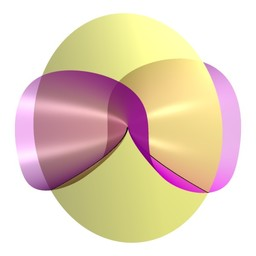
\includegraphics[width=1.2cm]{../../common/images/cuspe_cut}
        \end{tabular}
        &
        \begin{tabular}{@{}c@{}}
          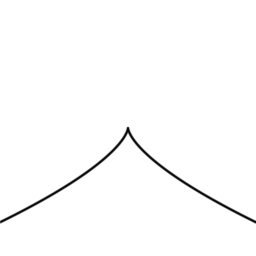
\includegraphics[width=1.2cm]{../../common/images/cuspe_rot}
        \end{tabular}
        &
        \begin{tabular}{@{}c@{}}
          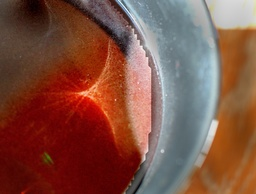
\includegraphics[width=1.4cm]{../../common/images/kuspe_detail_gross_heller}
        \end{tabular}
      \end{tabular}
    \end{center}
    \vspace*{-0.4em}
La imagen a la derecha muestra la cúspide que forma la luz reflejada
en una taza.

Una singularidad de tipo $A_k^{+-}$ se puede deformar en
    $\lfloor\frac{k+1}{2}\rfloor$
singularidades cónicas. En el caso $k=2$, por ejemplo, la
deformación es
    \[(1-a)x^3+ax^2+y^2-z^2=0.\]
Para $a=0$, se tiene la cúspide, y para valores pequeños de $a\neq0$ una
singularidad cónica:
    \vspace*{-0.6em}
    \begin{center}
      \begin{tabular}{@{}c@{\quad}c@{\quad}c@{}}
        \begin{tabular}{@{}c@{}}
          
\includegraphics[width=1.1cm]{../../common/images/A2pm_0}
        \end{tabular}
        &
        \begin{tabular}{@{}c@{}}
          
\includegraphics[width=1.1cm]{../../common/images/A2pm_1}
        \end{tabular}
        &
        \begin{tabular}{@{}c@{}}
          
\includegraphics[width=1.1cm]{../../common/images/A2pm_2}
        \end{tabular}
      \end{tabular}
    \end{center}
 
\end{surferPage}
